\documentclass{entcs}
\usepackage{entcsmacro}
\usepackage{graphicx}

%\documentclass{entcs} \usepackage{entcsmacro}
%\usepacka{graphicx}

\usepackage{latexsym,amsmath,epsfig,amssymb,graphics}
%\usepackage{latexsym,amsmath,epsfig,amssymb,graphics}
%\setlength{\textwidth}{6.50in}
%\setlength{\textheight}{8.5in}
%\setlength{\oddsidemargin}{-6mm}
%\setlength{\evensidemargin}{-6mm}
%\setlength{\topmargin}{0cm}
%\setlength{\footskip}{0.5cm}
%\setlength{\parindent}{0cm}
%\setlength{\parskip}{0.15cm}
%\newenvironment{FIG}
%        {\begin{figure}[h]\begin{center}}
%        {\end{center}\end{figure}}
\let \imply     \Rightarrow
\newcommand{\sizeimpl}{\hspace{4mm}}
\newcommand{\oomit}[1]{}
\newcommand{\dlceil}{\lceil\hspace{-0.05in}\lceil}
\newcommand{\drceil}{\rceil\hspace{-0.05in}\rceil}
\newcommand{\drceils}{\rceil\hspace{-0.05in}\rceil_{}^{*}}
\newcommand{\BBox}{\Box\hspace{-.14in}{\cdot}\:}
\newcommand{\BBoxx}{\Box\hspace{-.09in}{\cdot}\ }
\newcommand{\DDiamond}{\Diamond\hspace{-.14in}{\cdot}\:}
\newcommand{\DDiamondd}{\Diamond\hspace{-.09in}{\cdot}\ }
\newcommand{\Int}{\mbox{$\int$}}
\newcommand{\define}{\widehat{=}}
\newcommand{\Define}{\stackrel{\mbox{\small\rm def}}{=}}
\newcommand{\sep}[1]{\hspace{0.06in}#1\hspace{0.06in}}
\newcommand{\swedge}[1]{\bigwedge_{#1 \in \alpha}^{}}
\newcommand{\svee}[1]{\bigvee_{#1 \in \alpha}^{}}
\newcommand{\fracf}[1]{\lfloor l/T_{#1}\rfloor}
\newcommand{\fracc}[1]{\lceil l/T_{#1}\rceil}
%\newenvironment{definition}[1]{{\bf Definition}\ {\bf #1}\ \it}{\it}
%\newenvironment{proposition}[1]{{\bf Proposition}\ {\bf #1}\ \it}{\it}
\newcommand{\dempty}{\dlceil\;\;\drceil}
\newcommand{\dceil}[1]{\lceil #1\rceil}
\newcommand{\lead}[1]{\stackrel{ #1} {\rightarrow}}
\newcommand{\rsn}[1]{\mbox{{\small{\it\underline{#1}}}}}
\newcommand{\pstop}{$\Box\hspace{-.09in}\bullet$}
\newcommand{\ds}{\displaystyle}
%\newcommand{\lead}{\ds\Longrightarrow}
\newcommand{\lra}{\Longrightarrow}
\newcommand{\fracF}[1]{\left\lfloor\frac{l}{T_{#1}}\right\rfloor}
\newcommand{\pred}[1]{\dlceil #1 \drceil}
\newcommand{\mv}[1]{\overline{#1}}
\newcommand{\eqi}{\Leftrightarrow}
\def \p   {\prime}
\def \wh  {\;\widehat{}\;}
\def \emu   {\mbox{EM$\mu$ }}
\def \seqp  {{\cal{P}}^{s}}
\def \ord   {\mbox{${\cal{O}}$n}}
\def \msc   {\models_{sc}}
\def \flc  {\mbox{$\mathrm{FLC^+}~$}}
\def \bpa  {\mathrm{BPA}^{\epsilon}_{\delta}}
\def \implies {\Rightarrow}
\def \eqre    { \sim }
\newcommand{\dall}[1]{\lesssim \!\! #1 \!\!\succsim}
\newcommand{\di}[1]{{\langle} #1 {\rangle}}
%\newcommand{\di}[1]{<\!\!#1\!\!>}
\newcommand{\vrl}{\rule{0.5mm}{2mm}}
\newcommand{\hrl}[1]{\rule[1mm]{#1mm}{0.5mm}}
\newcommand{\CJ}{{\cal J}}
\newcommand{\CI}{{\cal I}}
\newcommand{\CV}{{\cal V}}
\newcommand{\IFF}{\Leftrightarrow}
\newcommand{\df}{\widehat{=}}
\newcommand{\always}[1]{\lceil #1 \rceil}
\newcommand{\ol}[1]{\overline{#1} }
%\newcommand{\dur}{\int}
\newcommand{\len}{\ell}
\newcommand{\sem}[2]{\mathcal{C}_{\rho}(#1)#2}
\newcommand{\ssem}[1]{{\cal{C}} (#1)}
\newcommand{\dsem}[2]{{\cal{C}}_{\rho[X\leadsto f]}(#1)#2}
\newcommand{\fracN}[2]{\frac{\displaystyle #1}{\displaystyle #2}}
\newcommand{\quo}[1]{{|\![\:} #1 {\:]\!|}}
\newcommand{\Nat}{{\mathbb N}}
\newcommand{\Real}{{\mathbb R}}
\newcommand{\modala}{a \hspace*{-3mm} \bigcirc}
\def\lastname{Naijun Zhan}


\begin{document}
\begin{frontmatter}
\title{Compositional Properties of Sequential Processes} 
\author{Naijun \ Zhan }
\address{ Lehrstuhl f\"{u}r Praktische Informatik II \\
           Facult\"{a}t f\"{u}r Mathematik und Informatik \\
           Mannheim Universit\"{a}t \\ 
           D7,27, 68163 
           Mannheim, Deutschland  \\
      Email: \{zhan\}@pi2.informatik.uni-mannheim.de }
\begin{abstract}  
It is widely agreed that
the modular method is one of the most effective methods
 to specify and verify complex systems in order to
avoid combinatorial explosion.
FLC ( Fixpoint Logic with Chop)  is
an important modal logic because of its expressivity and
logic properties, e.g., it is strictly more expressive
than the $\mu$-calculus.
In this paper, we study the compositionality of FLC, namely,
to investigate the connection between the connectives of the logic
and the constructors of programs.
To this end, we first extend FLC
with a nondeterministic
operator ``+'' (\flc for the extension) and then
establish a correspondence between the logic and
 the basic process algebra with deadlock and termination
 (abbreviated by $\bpa$).
 Finally, we show that as a by-product of the correspondence
 characteristic formulae for processes of $\bpa$ up to 
 strong (observational) bisimulation 
can be constructed compositionally directly from the syntax of
 processes.
\end{abstract}
 
\begin{keyword}
 chop operator, modal logic, compositionality,
verification, bisimulation, characteristic formula, process algebra
\end{keyword}
\end{frontmatter}

\section{Introduction}
There is a growing need for reliable methods in designing
correct reactive systems \cite{hp85} such as computer operating systems
and air traffic control systems.  These systems are characterized by
ongoing, typically nonterminating and highly nondeterministic behavior.
Such systems are often used to model ``{\em safety critical systems}''
like, e.g., air traffic control systems, nuclear reaction control
systems and so on. As any faulty behavior of such systems might imply
catastrophical consequences, proving the correctness of such systems
with respect to the expected behavior is inevitable.
There is a common agreement that
formal methods, such as modal and temporal logics \cite{MP92,stirling01}
 and process algebra \cite{bk85,Hoare86,Milner86a},
are effective and reliable methods to design these systems.

Because the complexity of  large systems is normally uncontrollable,
it is necessary that a method for developing
such systems is compositional (vertically or horizontally) 
in order to avoid combinatorial explosion in
specifying and verifying them, e.g.
 \cite{Hoare86,Milner86a,bk85,AH93,MCS00,bkp84,bkp85,tl88}.
The compositional method allows one to build up a large
system by composing existing systems with the defined
constructors and  reduce the
problem of correctness for a complex system to similar and simpler
correctness problems for the subsystems.

 FLC \cite{Olm99} is an extension of the $\mu$-calculus \cite{kozen83}
with the sequential composition operator --- ``chop'' (denoted by ``;'').
\cite{Olm99} pointed out that FLC is strictly more expressive than
the $\mu$-calculus because
\cite{ej91,jw96} proved that only ``regular'' properties can be defined in
the $\mu$-calculus, but characteristic formulae of context-free
processes can be defined in FLC. \cite{ls02,l02} investigated the
issue of FLC model checking.

The compositionality was stated in \cite{gs86a} as
one important requirement that should also be
satisfied by specification logic used in a
process algebraic setting, that is, any program
constructor cons corresponds to an operator {\bf cons} of the logic
such that
\begin{description}
\item (a)~ $P_i \models \phi_i$ for $i=1,\ldots, n$ implies
 $cons(P_1,\ldots, P_n) \models {\bf cons}(\phi_1,\ldots,\phi_n)$; 
 \item (b)~ $cons(P_1,\ldots,P_n) \models {\bf cons}(\phi_1,\ldots,\phi_n)$
  is the strongest assertion which can be deduced from
 $P_i \models \phi_i$ for $i=1,\ldots,n$.
\end{description}

It is clear that FLC does not meet the above conditions since
 $P$ meets $\phi$ and $Q$ satisfies $\psi$, but we can not
get any property that holds in the combined system $P+Q$ according
to $\phi$ and $\psi$ in FLC. In order to guarantee that a
specification logic satisfies the above conditions, we have two
alternatives: one is to show that for each constructor in process
algebra, a corresponding connective can be defined in the logic.
To our knowledge, until so far it is still an open problem if a
suitable ``+" is definable in classical modal logics; the other is
directly to introduce a connective, which exactly corresponds to
the constructor in process algebra,  into the logic like, e.g., in
\cite{gs86a,tl88} a non-deterministic choice ``+" is introduced
explicitly.

Besides, it is worth investigating the
connection between the sequential composition of process algebra
and the `chop' operator of FLC, but it seems no people to do
such a job up to now.

In this paper, 
we first extend FLC with a non-deterministic
operator ``+" (denoted by \flc\!).
Intuitively, $P \models \phi + \psi$ means that
 $P$ consists of two parts $P_1$ and $P_2$, which are
executed nondeterministically  such
that $P_1 \models \phi$ and $P_2 \models \psi$.
Then we show that the operators +, ; and $\nu X.$ in the logic relate to 
 +, ; and $rec\,x$ in process algebraic settings such as the basic process
algebra with termination and deadlock ($\bpa$ for short) respectively.
Thus, we can claim that the logic is compositional.

What's more, compositionality also makes many senses in practice for the following
reasons:
\begin{description}
\item i) It means one more step to the goal to exploit the structure
of  process terms for model checking. 
\item ii) It allows to give a precise and compact specification
of certain nondeterministic systems. 
\item iii) It is very easy to modify the specification of a system
when additional alternatives for the behavior of the system should
be admitted. 
\item iv) It enhances the possibility of modularity in model checking
  which is useful in redesigning of systems. 
\end{description}

 i) depends on if
it is possibly to work out a syntax-directed model checker for
 \flc \!. In fact, we believe that it may be done exploiting  
 the connection between \flc and $\bpa$ that is presented in this paper.
To explain the issues ii), iii) and iv), we present the following example:
Consider a car factory that wants to establish an
assembly line shown in the Figure~\ref{fg0},
\begin{center}
\begin{figure}[h]
% Bild
   \hspace*{2cm}
   \parbox[c]{80mm}{\scalebox{0.84}{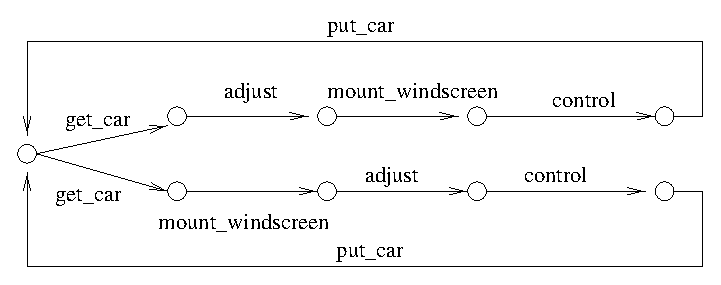
\includegraphics{con1.ps}}}
%   \vspace*{2mm}
 %%% \\
 \caption{The Process $P$\label{fg0}}
\end{figure}
\end{center}
%\vskip0.3cm
%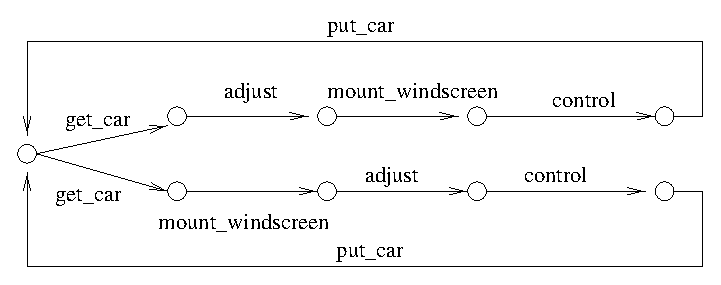
\includegraphics{con1.ps} ,
which we denote by the process $P$, for
one production step. If there is a car available for $P$ then
 $P$ will either get the car, adjust the motor, mount the
windscreen, control the car, and put the car on the
conveyer band or $P$ will  get the car,  mount the
windscreen, adjust the motor, control the car, and put it
back. Then $P$ may start again.
The first option can be specified by
\begin{eqnarray*}
 \mathrm{Spec_{1}} & \define &
    \mathrm{[get\_car];\di{adjust};\di{mount\_windscreen};\di{control};\di{put\_car}}  \\
                     &         & \wedge \mathrm{\di{get\_car};true,  } 
\end{eqnarray*}
whereas the second is described by
\begin{eqnarray*}
 \mathrm{Spec_{2}} & \define &
   \mathrm{ [get\_car];\di{mount\_windscreen};\di{adjust};\di{control};\di{put\_car}}\\
     &       &  \wedge \mathrm{\di{get\_car};true}.
\end{eqnarray*}
We are now looking for a specification that admits only such systems that
offer both alternatives and that can be easily constructed from
 $\mathrm{Spec_{1}}$ and $\mathrm{Spec_{2}}$.
Obviously, $\mathrm{Spec_{1}} \wedge \mathrm{Spec_{2}}$  is not
suitable whereas $\mathrm{Spec_{1}} \vee \mathrm{Spec_{2}}$ allows
for implementations that exhibit only one of the behavior.
 $\mathrm{Spec_{1}} + \mathrm{Spec_{2}}$ describes the behavior we
 have in mind and a system $P$ that offers this behavior repeatedly
 is described by
 \begin{eqnarray*} \mathrm{Spec} & \define & \nu
   X. (\mathrm{Spec_{1}}
   + \mathrm{Spec_{2}}); X. \end{eqnarray*}

It will be shown that 
 $rec\; x. (P_1 + P_2);x \models \mathrm{Spec}$
 in Example~\ref{exa-4} in Section 4, 
  where
\begin{eqnarray*}
 \mathrm{P_1} & \define &
    \mathrm{ get\_car;adjust; mount\_windscreen; control ; put\_car} \\
 \mathrm{P_2} & \define &
    \mathrm{ get\_car;mount\_windscreen;adjust;  control ; put\_car} .
\end{eqnarray*}
Let us now assume that the system specification should be modified to
allow for a third alternative behavior $\mathrm{Spec_{3}}$,
then this specification may be simply ``added'' to
form
 \begin{eqnarray*} \mathrm{Spec}^{\p} & \define & \nu
   X. (\mathrm{Spec_{1}}
   + \mathrm{Spec_{2}} + \mathrm{Spec_{3}}); X. \end{eqnarray*}
If we establish $P_3 \models \mathrm{Spec_{3}}$ then
 we obtain immediately that
 \begin{eqnarray*} rec\; x. (P_1 + P_2 + P_3 );x & \models &
  \mathrm{Spec}^{\p}. \end{eqnarray*}
In addition, if we have to modify $\mathrm{Spec}_{1}$ to
 $\mathrm{Spec_{1}^{\p}}$ such that
 $P_1^{\p}\models \mathrm{Spec_{1}^{\p}}$,
and obtain
\begin{eqnarray*} 
  rec\; x. (P_1^{\p} + P_2 + P_3 );x & \models & \nu X. (\mathrm{Spec_{1}^{\p}}
   + \mathrm{Spec_{2}} + \mathrm{Spec_{3}}); X. \end{eqnarray*}


The remainder of this paper is organized as follows: Some basic
notions are briefly reviewed in
Section 2; The syntax and semantics
of \flc are defined  in Section 3; Section 4
establishes a connection between the constructors of
$\bpa$ and the connectives of \flc\!;
In Section 5, an algorithm to construct
 a formula $\Psi_P$ for each process $P \in  \bpa$
 according to its syntax is presented
and we show that $\Psi_P;\surd$ is the
 characteristic formula of $P$ by the compositionality of \flc\!; Finally,
a brief conclusion is provided in Section 6.


\section{Preliminaries}
Let $Act$ be a finite set of (atomic) actions, ranged over by
 $a,b,c,\ldots$, and
 $\mathcal{X}$ be a countable set of process variables,
 ranged over by $x,y,z,...$.

%Transition systems are often used as models for concurrent
%programs and modal logics.
%A transition system is a triple ${\cal{T}} = (S, A,\rightarrow)$
%where $S$ is a set of states or processes,  $A$ is a set of
%actions, and $\rightarrow \subseteq S \times A \times S$.

Sequential process terms are those which do not involve parallelism and
communication, which are generated  by the following grammar:
\[
  E ::= \delta ~\mid~ \epsilon ~ \mid ~ x~\mid~ a~ \mid~ E_1;E_2~\mid E_1+E_2~
         \mid ~ rec \; x.E
 \]
We denote the above language by $\seqp$. Intuitively,
we consider that the elements of $\seqp$ represent programs;
 $\delta$ denotes a deadlocked process that cannot execute any
action and stays there for ever; $\epsilon$ denotes
a terminated process that can not proceed, but terminates at once;
the other constructors can be conceived as usual ones.

In the presence of the sequential composition operator ``;'' it is
common to use a special predicate $\mathcal{T}$ to evaluate the semantics
of the sequential composition operator ``;''. Let
 $\mathcal{T} \subset \seqp$ be the least set which contains
 $\epsilon$ and is closed under the rules:
\begin{description}
\item[$\bullet$]
 if $\mathcal{T}(E_1)$ and $\mathcal{T}(E_2)$ then
   $\mathcal{T}(E_1 ;E_2)$ and $\mathcal{T}(E_1+ E_2)$; and
\item[$\bullet$]
 if $\mathcal{T}(E)$ then
 $\mathcal{T}(rec\; x. E)$.
\end{description}

\noindent
\emph{Convention: }
 For the sake of simplicity, as a well-formedness
condition, expressions like $E=E_1+E_2$ in which
 $\mathcal{T}(E_1)$ and $\neg \mathcal{T}(E_2)$ or
 $\neg \mathcal{T}(E_1)$ and $\mathcal{T}(E_2)$  are
prohibited.

An occurrence of a variable $x \in \mathcal{X}$ is called {\em free} in an
expression $E$ iff it does not occur within any sub-term of the form
 $rec \; x. E^{\p}$, otherwise called {\em bound}.
We will use  $fn(E)$ to stand for  all variables which have some
free occurrence  in $E$,
 and $bn(E)$ for all bound variables which have some bound occurrence in $E$.
A variable $x \in \mathcal{X}$ is called {\em  guarded} within a
term $E$
 iff every occurrence of $x$ is within a
 sub-term $F$ where $F$ lies in a subexpression $F^*;F$ such that
 $\neg \mathcal{T}(F^*)$. A term $E$ is called \emph{guarded} iff
 all variables occurring in it are guarded.
The set of all closed and guarded terms of $\seqp$ essentially corresponds to
 {\em basic process algebra ($\mathrm{BPA}$)} with the terminated process
 $\epsilon$ and the deadlocked process $\delta$, denoted by
 $\bpa$, ranged over by $P,Q,\ldots$.
 $\mathrm{BPA}$ is a sub-fragment of $\mathrm{ACP}$ \cite{bk85}.

\begin{example} The expressions $a;x, a;(b+x), rec\;x. (a+b);x;(y+z), \epsilon, \delta$
are guarded whereas $x, a+x$ are unguarded.
\end{example}

An operational semantics of $\seqp$
is given by the following inference rules:
\medskip
\begin{center}
%\begin{tabular}{c}
 \begin{tabular}{llll}
 Act~ & $\fracN{}{a \lead{a} \epsilon}$   &
 Rec~~ &
     $\fracN{E_1[rec.x E_1 /x] \lead{a} E_1^{\p}}{rec \; x. E_1  \lead{a}
     E_1^{\p} }$  \\
 Seq-1 &
   $\fracN{E_1 \lead{a} E_1^{\p}}{E_1;E_2  \lead{a} E_1^{\p};E_2}$ \hspace{1.cm} &
%  \end{tabular}\\[.5cm]
%\begin{tabular}{ll}
 Seq-2 ~~&
 $\fracN{E_2 \lead{a} E_2^{\p} \mbox{ and } \surd(E_1)}{E_1;E_2
     \lead{a} E_2^{\p}}$  \\
% \end{tabular}  \\
 Nd~~ ~~&   $\fracN{E_1 \lead{a} E_1^{\p}}
 %~~ E_2 \mbox{ is guarded or $E_2$ is closed} }
{E_1 + E_2
     \lead{a} E_1^{\p} \mbox{ and }  E_2 + E_1 \lead{a} E_1^{\p}}$ &&
\end{tabular}

 \end{center}

\begin{definition} \label{def-equi}
A binary relation ${\cal{S}} \subseteq \bpa \times \bpa$
 is called a strong bisimulation if $(P,Q) \in {\cal{S}}$  implies
\begin{itemize}
\item $\surd(P)$ iff $\surd(Q)$; and
\item whenever $P \lead{a} P^{\p}$ then,
  for some $Q^{\p}, Q\lead{a} Q^{\p}$
  and $(P^{\p},Q^{\p}) \in {\cal{S}}$,
for any $a \in Act$; and
\item whenever $Q \lead{a} Q^{\p}$ then,
  for some $P^{\p}, P\lead{a} P^{\p}$
  and $(P^{\p},Q^{\p}) \in {\cal{S}}$ for any $a \in Act$.
\end{itemize}
Given two processes $P,Q \in \bpa$, we say
 $P$ and $Q$ are strongly bisimilar, written $P \sim Q$, if
 $(P,Q) \in {\cal{S}}$ for some strong bisimulation ${\cal{S}}$.
\end{definition}

 We can  extend the definition of $\sim$ over $\seqp$ as: 
Let $E_1,E_2 \in \seqp$, and
 $fn(E_1)\cup fn(E_2) \subseteq \{x_1,\ldots, x_n\}$.
 If $E_1\{P_1/x_1,\ldots,P_n/x_n\} \sim E_2\{P_1/x_1,\ldots,P_n/x_n\}$ for any
 $P_1,\ldots,P_n \in \bpa$, then  $E_1\sim E_2$.

%\medskip

\cite{AH92} proved that the following proof system
for  $\bpa$  is complete
 \footnotemark \footnotetext{The proof system for $\bpa$
  presented in this paper
is a little different from the one in \cite{AH92}. But \cite{AH92} pointed out
that the variant is still complete. } :
\[
\begin{array}{llll}
\mathrm{A0}~~ &  E_1+E_2 =  E_2+E_1 ~~~ &
\mathrm{A1} ~~ & (E_1+E_2)+E_3  =  E_1+(E_2+E_3) \\
%\end{array}\]
%\[\begin{array}{llll}
\mathrm{A2} &  E+E  =  E  &
\mathrm{A3} & (E_1+E_2);E_3  =   (E_1;E_3)+ (E_2;E_3) 
\end{array} \]
\[\begin{array}{llll}
%          &  &   &                                                   
\mathrm{A4} ~~ & (E_1;E_2);E_3  =   E_1;(E_2;E_3) ~~&
\mbox{A5} & rec\;x. E    =    E\{rec\;x. E/x\}\\
\mathrm{A6} &  E+\delta  =  E  &
\mathrm{A7} &  \delta;E  =  \delta \\
\mathrm{A8} &  E;\epsilon  =  E  &
\mathrm{A9} & \epsilon; E   =  E
\end{array} \]

Also in \cite{AH92}, the following lemma was shown.
\begin{lemma} \label{lem-cong}
For any $P \in \bpa$,
 $P \eqre \sum_{a\in Act}\sum_{j=1}^{i_a}a;Q_{a,j}$ or
 $P \eqre \delta$, where $Q_{a,j} \in \bpa$.
Note that if for all $a\in Act$, $i_a < 1$ then 
 $\sum_{a\in Act}\sum_{j=1}^{i_a} a; Q_{a,j}$ will be abbreviated as 
$\epsilon$.  
\end{lemma}

\noindent
\emph{Notations: }From now on, we use $\mathcal{A} \; op \; \mathcal{B}$ to stand for
 $\{E_1 \; op \; E_2 \mid E_1 \in \mathcal{A} \mbox{ and }E_2 \in \mathcal{B}\}$,
 $\mathcal{A}\; op \; E $ for   $\mathcal{A}\; op \; \{E \}$,
where $E \in \seqp, \mathcal{A}\subseteq \seqp, \mathcal{B}\subseteq\seqp$,
and $op \in \{+,;\}$.

\section{FLC with Nondeterministic Operator ``+'' (\flc\!) }
FLC is due to Markus M\"{u}ller-Olm \cite{Olm99}, which is
an extension of the modal $\mu$-calculus,  can express
 non-regular properties. It is therefore strictly
more expressive than the $\mu$-calculus, since \cite{ej91,jw96} proved that
only regular properties can be defined in the $\mu$-calculus.
Here, we extend FLC with a nondeterministic operator ``+'', which is similar
to the one presented in \cite{gs86,tl88}, in order to
define the composed property according to the ones for
 the two components which can be executed nondeterministically.
Intuitively, $P \models \phi_1 + \phi_2$
 means that $P$ consists of $P_1$ and $P_2$ which are
executed nondeterministically such that
 $P_1$ satisfies $\phi_1$ and $P_2$ meets $\phi_2$.

\subsection{Syntax and Semantics}
Let $X, Y, Z, \ldots $ range over an infinite
set $\mathit{Var}$ of {\em variables},
 $true$ and $false$ be propositional constants as usual,
 and $\surd$ for another special propositional constant
 that is used to
indicate if a process is terminated.

Formulae of \flc are generated by the following rules:
\begin{eqnarray} 
 \phi & ::= & true  \mid false \mid \surd \mid term \mid  X \mid [a] \mid \di{a}
                 \mid \phi_1 \wedge \phi_2
      \mid  \phi_1 \vee \phi_2  \mid \nonumber \\[2mm]
      &     & \phi_1 ; \phi_2 \mid
      \phi_1 + \phi_2 \mid
      \mu X. \phi \mid \nu
      X. \phi  \nonumber
\end{eqnarray}
where $X \in Var$ and $a \in Act$.

In the sequel, we use $\modala$ to stand for $\di{a}$ or $[a]$,
 $p$ for $\mathit{true,false}$ or $\surd$,
 and $\sigma$ for $\nu$ or $\mu$.

As in the modal $\mu$-calculus, the two {\em fixpoint operators}
 $\mu X$ and $\nu X$ bind the respective variable $X$ and we will
apply the usual terminology of {\em free} and {\em bound occurrences } of variables
in a formula, {\em closed} and \emph{open} formulae etc.
 We will use $fn(\phi)$ to stand for all variables which have some free
 occurrence in
 $\phi$ and $bf(\phi)$ for all variables that have some
bound occurrence in $\phi$.
 We say that $X$ is guarded in $\phi$ if each
occurrence of $X$ is preceded with $\modala$ or $p$ via ``;".
If all variables in $\phi$ are guarded, then $\phi$ is called
\emph{guarded}.

\begin{example} Formulae
 $\di{a};X, \nu X. (\di{a}\vee \di{b});X;(Y+Z), \mathit{false};X$ are guarded, but
 $X, \di{a}\wedge X, \mu X.(X+Y)\vee [a]$ are not guarded.
\end{example}

As in \cite{Olm99},
formulae are interpreted as
a {\em monotonic predicate transformer} which
 is simply a mapping $f: 2^{\bpa} \rightarrow 2^{\bpa}$ which is
monotonic w.r.t. the inclusion ordering on $2^{\bpa}$.
We use $\mathrm{MPT_T}$ to represent all these monotonic predicate transformers
over $\bpa$.
 $\mathrm{MPT_T}$ together with the inclusion ordering defined by
 \[ f \subseteq f^{\p} \mbox{ iff } f(\mathcal{A}) \subseteq f^{\p}(\mathcal{A}) \mbox{ for
   all } \mathcal{A} \subseteq \bpa \]
forms a complete lattice. We denote the join and meet operators by
 $\sqcup$ and $\sqcap$.
By Tarski-Knaster Theorem, the least and greatest
fixed points of monotonic functions:
\[ (2^{\bpa} \rightarrow 2^{\bpa}) \rightarrow
 (2^{\bpa} \rightarrow 2^{\bpa})\] exist.
They are used to interpret the fixed point formulae of \flc\!.

The meaning of $true$ and $false$ are interpreted in the standard way,
 i.e.
by $\bpa$ and $\emptyset$ respectively.
The meaning of  $\surd$ is to map any set of processes
to the subset of $\bpa$ in which all terminated processes
are contained.
So, a process $P$ meets $\surd$ iff $\mathcal{T}(P)$.
 $term$ is interpreted as an identity.
Because $\epsilon$ and $\delta$ have different behavior in
 the presence of $;$, they should be distinguished by \flc\!.
To this end,  $[a]$ of \flc is interpreted
 as a function that maps any set of processes $\mathcal{A}$
 to the set in which each process is not terminated and
every $a$-successor of the process must be contained in
 $\mathcal{A}$. This
is different from the meaning
 of $[a]$ given in FLC. Therefore, according to our interpretation,
 $P \models [a]$ only if $\neg \mathcal{T}(P)$. Whereas, $P$ always meets
 $[a]$  for any $P \in \bpa$ in FLC. So,
 it is easy to show that
 $\epsilon$ does not satisfy $\bigwedge_{a \in Act} [a];false$,
while $\bigwedge_{a \in Act} [a];false$ is the characteristic formula
 of  $\delta$.
The meaning of variables is given by an \emph{environment} $\rho$
:  $var \rightarrow (2^{\bpa} \rightarrow 2^{\bpa})$ that
assigns variables to monotonic functions of sets to sets.
 $\rho[X \leadsto f]$ agrees with $\rho$ except for
associating $f$ with $X$.

\begin{definition} \label{def-sem}
Given an environment $\rho$, the meaning of
 a formula $\phi$, denoted by
 ${\cal{C}}_{\rho}(\phi)$, is inductively defined as
follows:
 \begin{eqnarray*}
 \sem{true}{(\mathcal{A})}& = &\bpa \\
 \sem{false}{(\mathcal{A})} &= &\emptyset \\%[.1mm]
 \sem{\surd}{(\mathcal{A})} &= &\{P\in \bpa \mid \mathcal{T}(P)\}\\%[.1mm]
% \sem{p}{(E)}& =  & {\cal{I}}(p)  \\[2mm]
 \sem{term}{(\mathcal{A})} & = & \mathcal{A} \\%[.1mm]
 \sem{X}{} & = &\rho(X) \\
 \sem{[a]}{(\mathcal{A})} & = & \{ P \in \bpa \mid \neg
\mathcal{T}(P)\wedge \forall P^{\p}\in \bpa. P \lead{a} P^{\p} \imply
 P^{\p} \in \mathcal{A}\} \\%[.1mm]
 \sem{\di{a}}{(\mathcal{A})} & = & \{ P\in \bpa \mid \exists P^{\p}\in \bpa. P\lead{a} P^{\p} \wedge
 P^{\p} \in \mathcal{A}\}\\%[.1mm]
\end{eqnarray*}
%\\[.1mm]
\begin{eqnarray*}
 \sem{\phi_1\wedge\phi_2}{(\mathcal{A})} & = & \sem{\phi_1}{(\mathcal{A})} \cap
 \sem{\phi_2}{(\mathcal{A})} \\%[.1mm]
 \sem{\phi_1\vee\phi_2}{(\mathcal{A})} & = & \sem{\phi_1}{(\mathcal{A})} \cup
 \sem{\phi_2}{(\mathcal{A})}\\%[.1mm]
 \sem{\phi_1 ; \phi_2}{} & = & \sem{\phi_1}{} \cdot
 \sem{\phi_2}{}  \\%[.1mm]
 \sem{\phi_1 + \phi_2}{(\mathcal{A})} & = & \{ P\in \bpa \mid \exists P_1,P_2\in \bpa. P \eqre P_1+P_2 \wedge \\
                                      &    & ~~~~~~~~~~~~~~~~~ P_1 \in
 \sem{\phi_1}({\mathcal{A}})  \wedge P_2 \in
 \sem{\phi_2}{(\mathcal{A})}\}  \\%[.1mm]
 \sem{\mu X. \phi}{} & = & \sqcap\{f \in \mathrm{MPT_T} ~\mid ~ \dsem{\phi}
 \subseteq f \} \\%[.1mm]
 \sem{\nu X. \phi}{} & = & \sqcup\{f \in \mathrm{MPT_T} ~\mid ~ \dsem{\phi}
 \supseteq f \}
  \end{eqnarray*}
where $\mathcal{A} \subseteq \bpa$, and
 $\cdot$  stands for the compositional operator over functions.
\end{definition}

As the meaning of a closed formula $\phi$ is independent of any
environment, we sometimes write $\ssem{\phi}$ for $\sem{\phi}{}$,
where $\rho$ is an arbitrary environment. We also abuse $\phi(\mathcal{A})$
to stand for $\sem{\phi}{(\mathcal{A})}$ if $\rho$ is clear from the
context.

The set of processes {\em satisfying} a given closed formula $\phi$ is
 $\phi(\bpa)$. A process $P$
is said to
satisfy $\phi$ iff $P \in \sem{\phi}{(\bpa)}$ for some
 environment $\rho$,
denoted by $P \models_{\rho} \phi$. If $\rho$ is clear from the 
context, we directly write $P \models \phi$. $\phi \implies \psi$ means that
 $\sem{\phi}{(\mathcal{A})} \subseteq \sem{\psi}{(\mathcal{A})}$
for any $\mathcal{A} \subset \bpa$  and any $\rho$.
 $\phi \eqi \psi$ means $(\phi \implies \psi) \wedge (\psi \implies \phi)$.
The other notations can be defined in a standard way.

%\begin{proposition} \label{prop-1}
% $\sigma X. \phi ~ \eqi ~ \phi\{\sigma X.\phi /X\}$.
%\end{proposition}


 Given a formula $\phi$, the set of sub-formulae
  at the end of $\phi$, denoted by $\mathrm{ESub(\phi)}$, is:
     $\{\phi \}$ if $\phi = p, term,X$ or $\modala$;
   $\mathrm{ESub(\phi_1)} \cup \mathrm{ESub(\phi_2)}$
 if  $\phi = \phi_1 \; op \; \phi_2$  where
              $op\; \in \{\wedge,\vee,+\}$; if $\phi = \phi_1 ; \phi_2$
       then if $\tau \not \in \mathrm{ESub(\phi_2)}$ 
               then $\mathrm{ESub(\phi_2)}$ else  
       $(\mathrm{ESub(\phi_2)}-\{\tau\}) \cup \mathrm{ESub(\phi_1)}$;
     $\mathrm{ESub(\phi^{\p})}$ if  $\phi = \sigma X. \phi^{\p}$.
When we say that $\surd$ only occurs at the end of $\phi$ it  means that
 $\surd$ only can be in $\mathrm{ESub(\phi)}$ as a sub-formula of
 $\phi$.

\noindent
{\em Convention: }In the sequel, we assume the binding precedence
among the operators of the logic as follows:
 $``\nu X" = ``\mu X" > ``;" > ``+" > ``\vee" = ``\wedge" > ``\imply" = ``\eqi"$.

\subsection{Some Theorems  for \flc}
In this subsection, we prove some theorems for \flc which will be
used in the later.

In fact, we can prove that all properties on FLC shown in \cite{Olm99}
 are still true for \flc\!, e.g.,
 \flc is strictly more expressive than the $\mu$-calculus,
 \flc is decidable for finite-state processes and undecidable
 for context-free processes and so on.

Besides,
we can show that \flc has the tree model property, viz %Our proof is
%completely different from the one presented in
% \cite{ls02} to prove that FLC has such property.
\begin{theorem} \label{the-tree}
Given $P, Q \in \bpa$, and
 $P \sim Q$, then for any closed formula $\phi$ of \flc\!, $P \models \phi$ iff
 $Q \models \phi$.
\end{theorem}

\begin{definition}
We define a subclass of \flc\!, denoted by $\mathcal{N}$, as follows:
\begin{eqnarray*}
  \phi & ::= & p \mid \modala \mid \phi \wedge \phi \mid \phi + \phi
 \mid \modala;\psi \end{eqnarray*}
where $a\in Act, \psi \in \flc$\!.
\end{definition}

 By the definition of the semantics of \flc\!,
 $\phi; true \implies \psi;true$ means that for
any process $P$ and environment $\rho$, $P \models_{\rho} \phi$ 
implies $P \models_{\rho} \psi$.
 For convenience, we abbreviate $\phi; true \implies \psi;true$ by
 $\phi \rightarrow \psi$, and  $\phi; true \eqi \psi;true$  by
 $\phi \leftrightarrow \psi$.

The following theorem indicates the relationships among the propositional
letters, connectives of \flc\!.
\begin{theorem} \label{the-a}
\[\begin{array}{llll}
\mathrm{N1} & term ;     \phi \eqi  \phi ; term \eqi\phi  &
\mathrm{P1} & p ; \phi \eqi p \\
\mathrm{P2} & \phi + false \eqi false &
\mathrm{P3} & p + p \eqi p  \\[.5mm]
\mathrm{P4} & \di{a};false \eqi false  &
\mathrm{T1} & \surd \vee [a];true \eqi true \\%[.5mm]
\mathrm{T2} & \surd \wedge [a];true \eqi false  &
\mathrm{S1} & \phi + \psi \eqi \psi + \phi \\%[.5mm]
%\end{array}\]
%\[\begin{array}{llll}
\mathrm{S2} & (\phi + \psi)+\varphi \eqi \phi+(\psi+\varphi) &
\mathrm{S3} &  \phi + \phi \leftrightarrow \phi \mbox{ if } \phi \in \mathcal{N} \\%[.5mm]
\mathrm{SI} & \phi + (\psi \wedge \varphi)
        \implies (\phi + \psi)\wedge (\phi + \varphi) &
\mathrm{SD} & \phi + (\psi \vee \varphi) \eqi (\phi + \psi) \vee (\phi + \varphi) \\%[.5mm]
\mathrm{SC} & (\phi + \psi) ; \varphi \eqi (\phi;\varphi) + (\psi;\varphi) &
\mathrm{C1} & \phi;\psi \rightarrow \phi \\%[.5mm]
\mathrm{C2} & (\phi ; \psi) ; \varphi  \eqi\phi ; (\psi ; \varphi) &
\mathrm{IC} & (\phi \wedge \psi) ; \varphi  \eqi (\phi ; \varphi)
         \wedge (\psi ; \varphi) \\%[.5mm]
\mathrm{DC} &  (\phi \vee \psi) ; \varphi  \eqi (\phi ; \varphi) \vee (\psi ;\varphi) &
\mathrm{SD} & [a];\phi_1 + [a];\phi_2 \leftrightarrow [a];(\phi_1\vee \phi_2)
\end{array} \]
\end{theorem}

The following theorem says that ``;'' and ``+'' both are monotonic.
\begin{theorem} \label{the-b}
 \begin{description}
\item[(i)]
 If ${\displaystyle \phi \implies \psi}$ then
  ${\displaystyle \phi;\varphi \implies \psi;\varphi}$  and
 $\varphi;\phi \implies \varphi;\psi$; and
\item[(ii)]
If ${ \displaystyle\phi_1 \implies \phi_2 \mbox{ and } \psi_1 \implies  \psi_2}$
then ${ \displaystyle \phi_1 + \psi_1 \implies \phi_2 +  \psi_2}$.
\end{description}
\end{theorem}


By extending the tableau based model checker for
FLC given in \cite{ls02} with a rule for ``+'', namely
 \begin{eqnarray*}(+)~~~ &  \frac{\displaystyle (\mathcal{E},\mathcal{F})
     \vdash \phi_1 + \phi_2} {\displaystyle
      (\mathcal{E}_1,\mathcal{F}) \vdash \phi_1 ~~
      (\mathcal{E}_2,\mathcal{F})\vdash \phi_2}
    &~~ ~ \mathcal{E} = \mathcal{E}_1+ \mathcal{E}_2
 \end{eqnarray*}
where $\mathcal{E},\mathcal{E}_1,\mathcal{E}_2,\mathcal{F}\subseteq \bpa$,
we can get a model checker for $\flc$\!, whose complexity is same as the one
of the model-checker of FLC presented in \cite{ls02}.

\section{Correspondence between \flc and $\bpa$}
In this section, we discuss how to derive composite properties
for a sequential process from those of its components.

\subsection{Nondeterminism}
It is clear that the connection between ``+'' of $\bpa$
and ``+'' of \flc can be expressed as follows:
\begin{theorem}\label{the-non}
\begin{description}
\item[(i)] For any $P,Q \in \bpa$, if
 $P \models \phi$ and $Q \models \psi$ then
 $P + Q \models \phi + \psi$;
\item[(ii)] For any $R \in \bpa$,  if
 $R \models \phi + \psi$ then
 there exist $P,Q \in \bpa$ such that
 $R \eqre P + Q$, $P \models \phi$ and $Q \models \psi$.
\end{description}
\end{theorem}
%\begin{proof} It is obvious. \hfill $\dashv$ \end{proof}


\subsection{Sequential Composition}
In this subsection, we show that the sequential composition of
process algebra  can be characterized by the chop operator.

Normally,  $P \models \phi$ and $Q \models \psi$,
 but $P;Q \not \models \phi ; \psi$ because
 possibly $\phi$ only describes some partial executions of
 $P$.
For example, let $P = a;b$, $Q = c;d$.
 It's obvious that $P \models \di{a}$ and $Q \models \di{c}$,
but $P;Q \not \models \di{a} ; \di{c}$.
So, we require that the property of the first operand of
 $;$ must specify full executions of the corresponding process, that is,
 $P \models \phi; \surd$. This is similar to the premise of the rule
 Seq-2 that
only after the first segment $P$ of ; finishes the executing, then
the second one can be performed.

Another issue is that by the definition of the semantics of
 $\seqp$, $\epsilon;P \sim P$. Therefore,
 the properties concerning intermediate terminations should be
omitted in the resulting formula.
Otherwise, the composed property does not hold in the
combined system. E.g., let $P = a;\epsilon$ and
 $Q = b;\delta$, $\phi = \di{a};\surd $,
and $\psi = \di{b}$.
 It's obvious that $P \models \phi;\surd$ and
  $Q \models \psi$ but
 $P;Q \not \models \phi ; \psi$. So, we will replace $\surd$ occurring
 in $\phi$ with $term$ since $term$ is a neutral element of the chop.
This is in accordance with
 that $\epsilon$ is a neutral element of
the sequential composition ``;'' (See the axioms A8 and A9).

Besides, since $\phi\{term/\surd\};\psi$ will be as a specification of
 $P;Q$, it is possible that $\surd$ as a sub-formula of $\phi$
makes the sub-formulae of $\phi$ followed it by ; no sense during
calculating the meaning of $\phi$ by
   P1, but
the sub-formulae play a nontrivial role during calculating the
meaning of
 $\phi \{term/\surd\};\psi$. E.g. $\epsilon \models \surd ; [a];\di{b}$ and
 $a;c \models \di{a};\di{c}$, but
 $\epsilon;(a;c) \not \models (term;[a];\di{b});(\di{a};\di{c})$.
So, we require that $\surd$ only can appear at the end of
 $\phi$ as a sub-formula. In fact, such a requirement is
reasonable because
 all formulae can be transform to such kind
of the form equivalently by Theorem~\ref{the-a}.

In a word, we have the following theorem on the sequential composition
 ``;'':
\begin{theorem} \label{the-seq}
If $\surd$ only occurs at the end of $\phi$ as a sub-formula,
 $P \models \phi;\surd$ and $Q\models \psi$ then
 $P;Q \models \phi\{term/\surd\}; \psi$.
\end{theorem}

\begin{remark}
Generally speaking, the converse of Theorem~\ref{the-seq} is not
valid,  e.g.
 $(a;b;c+ a); (c;d) \models \di{a} ; (\di{b} ; \di{c};\di{c})$,
but we can not conclude that
 $a;b;c +a \models \di{a};\surd$ and $c;d \models \di{b} ;\di{c};\di{c}$.
\end{remark}

\subsection{Recursion}
In this subsection, we will study how to relate $rec\; x$ to
 $\nu X$. So, in this subsection, all fixed point operators occurring
 in formulae
 will refer to $\nu$ if no otherwise stated.
To this end,   we
firstly define a relation called syntactical confirmation
 between processes and formulae, with the type
 $\seqp \times FLC^+ \mapsto \{\mathrm{true, false}\}$, denoted by $\msc$.

\begin{definition} \label{def-msc}
 Given a formula $\phi$, we associate a map from $2^{\seqp}$
 to $2^{\seqp}$ with it, denoted by $\widehat{\phi}$, constructed
   by the following rules:
 \begin{eqnarray*}
  \widehat{\surd}(\mathcal{E}) & \define & \{E \mid E \in \seqp
      \wedge \mathcal{T}(E) \} \\%[.5mm]
  \widehat{\mathit{true}}(\mathcal{E}) & \define & \seqp  \\%[.5mm]
  \widehat{\mathit{false}}(\mathcal{E}) & \define & \emptyset  \\%[.5mm]
  \widehat{term}(\mathcal{E}) & \define & \mathcal{E}  \\%[.5mm]
  \widehat{X}(\mathcal{E}) & \define & \{x;E \mid E \in \mathcal{E}\}  \\%[.5mm]
  \widehat{\di{a}}(\mathcal{E}) & \define & \{E \mid \exists E^{\p} \in \mathcal{E}.
      E\lead{a} E^{\p} \} \\%[.5mm]
  \widehat{[a]}(\mathcal{E}) & \define & \{E \mid \neg \mathcal{T}(E) \wedge
       E \mbox{ is guarded } \wedge \forall E^{\p}.
      E\lead{a} E^{\p} \implies E^{\p} \in \mathcal{E}\} \\%[.5mm]
  \widehat{\phi_1\wedge \phi_2}(\mathcal{E}) & \define &
      \widehat{\phi_1}(\mathcal{E}) \cap \widehat{\phi_2}(\mathcal{E}) \\%[.5mm]
 \widehat{\phi_1\vee \phi_2}(\mathcal{E}) & \define &
      \widehat{\phi_1}(\mathcal{E}) \cup \widehat{\phi_2}(\mathcal{E}) \\%
  %\\%[.5mm]
 \widehat{\phi_1 + \phi_2}(\mathcal{E}) & \define & \{E\mid \exists
      E_1,E_2. E = E_1+E_2\wedge
      E_1 \in \widehat{\phi_1}(\mathcal{E}) \wedge E_2\in
              \widehat{\phi_2}(\mathcal{E})\} \\%[.5mm]
 \widehat{\phi_1 ; \phi_2}(\mathcal{E}) & \define &
      \widehat{\phi_1}\cdot\widehat{\phi_1}(\mathcal{E}) \\ %[.5mm]
%\end{eqnarray*}
%\begin{eqnarray*}
 \widehat{\sigma X. \phi}(\mathcal{E}) & \define & \{(rec\;x. E_1); E_2
      \mid E_1 \in \widehat{\phi}(\{\epsilon\}) \wedge E_2 \in
      \mathcal{E}\}
\end{eqnarray*}
where $\mathcal{E} \subseteq \seqp$.

 $\msc(E,\phi) = \mathrm{true}$ iff $E \in \widehat{\phi}(\{\epsilon\})$; otherwise,
 $\msc(E,\phi) = \mathrm{false}$.
Hereinafter, we denote $\msc(E,\phi) = \mathrm{true}$ by
 $E \msc \phi$ and $\msc(E,\phi) = \mathrm{false}$ by  $E \not \msc \phi$.
\end{definition}

Informally, $P\msc \phi$ means that
 $P$ and $\phi$ have a similar syntax, e.g.
 \[rec\;x. [(a;x;x;b) + c] \msc \nu X. [(\di{a};X;X;\di{b}) \wedge \di{c}].\]

The following theorem states that $\msc$ itself is
 compositional too.
\begin{theorem} \label{the-msc-com}
Let $\surd$ only appear at the end of $\phi_1$, $\phi_2$ and $\phi$ as
a sub-formula. Then,
\begin{description}
\item i)~ if $E_1 \msc \phi_1$ and $E_2 \msc \phi_2$ then
      $E_1 + E_2 \msc \phi_1 + \phi_2$;
\item ii)~ if $E_1 \msc \phi_1$ and $E_2 \msc \phi_2$ then
      $E_1 ; E_2 \msc \phi_1\{term/\surd\} ; \phi_2$;
\item iii)~ if $E \msc \phi$ then $rec\; x. E \msc \sigma X. \phi\{term/\surd\}$.
\end{description}
\end{theorem}

\begin{example} \label{example-1}
Let $E_1 \define (a;x;x) + d$,
 $E_2\define x;(b+c);y$, $E_3\define a;b;c$,
 $\phi\define \di{a};X;X$, \\ $\psi \define  X; \di{b}; Y$
and  $\varphi \define [a];\di{b};\di{c}$. It's obvious that
 $E_1 \msc \phi$, $E_2\msc \psi$, $E_3\msc \varphi$,
 $E_1 + E_3 \msc \phi + \psi$,
 $E_3;(E_1+E_3) \msc \varphi;(\phi+\psi)$ and
 $rec\;x.\;rec\;y.E_3;(E_1+E_3) \msc \nu X. \nu Y. (\varphi;(\phi+\psi))$
by Definition~\ref{def-msc}.
\end{example}


The following lemma indicates that replacing $\msc$ with 
 $\models$, the relation between processes and formulae 
is preserved by substitution, i.e.,
\begin{lemma} \label{lem-D}
Let $fn(E) \subseteq \{x_1,\ldots,x_n\}$,
 $fn(\psi)\subseteq \{X_1,\ldots,X_n\}$ .
If $E \msc \psi$ and $P_i \models \phi_i;\surd$ where $\surd$
does not occur neither in $\phi_i$ for $i\in \{1,\ldots,n\}$ nor in $\psi$, then
 \begin{eqnarray*}
 E\{P_1/x_1,\ldots,P_n/X_n\} & \models
 &\psi\{\phi_1/X_1,\ldots,\phi_n/X_n\};\surd.
\end{eqnarray*}
\end{lemma}

Theorem~\ref{the-sequential} establishes a connection between
 $\msc$ and $\models$, so that we can relate $rec\; x$ to
 $\nu X$. For instance, in the above example, we get
 \[rec\;x.\;rec\;y.E_3;(E_1+E_3) \models \nu X. \nu Y. (\varphi;(\phi+\psi)).\]

\begin{theorem}\label{the-sequential}
 If $P \in \bpa$, $\surd$ only occurs at the end of  $\phi$ 
 and $P \msc \phi$, then
 $P \models \phi;\surd$.
\end{theorem}

In order to demonstrate how to apply the compositionality of \flc to 
simplify  the verification of reactive systems, we continue the example of a 
car factory given in Section 1.
\begin{example} \label{exa-4}
In the example, by Definition~\ref{def-msc},
it is easy to show that $\mathrm{P_1} \msc \mathrm{Spec_1}$ and
 $\mathrm{P_2} \msc \mathrm{Spec_2}$.
Therefore, we have
 \begin{eqnarray*} rec\;x. (\mathrm{P_1+P_2}); x & \msc&
                   \nu X. (\mathrm{Spec_1 + Spec_2});X
 \end{eqnarray*} by Theorem~\ref{the-msc-com}.
Furthermore, it follows that
 \begin{eqnarray*} rec\;x. (\mathrm{P_1+P_2}); x & \models &
                   \nu X. (\mathrm{Spec_1 + Spec_2});X
 \end{eqnarray*} by Theorem~\ref{the-sequential}.
That is,
 \begin{eqnarray*} P & \models & \mathrm{Spec}. 
\end{eqnarray*} 
\end{example}

\section{Constructing Characteristic Formulae of Sequential
  Processes}
Given an equivalence or
preorder $\preceq$ over processes,
the characteristic formula for a process $P$ up to $\preceq$ 
is a formula $\phi_P$ such that given a process $Q$,
 $Q \models \phi_P$ if and only if $Q \preceq P$.
Characteristic formulae
can be used to relate equational reasoning about processes to reasoning
in a modal logic, and therefore to allow proofs about processes
to be carried out in a logical framework.
\cite{gs86} proposed an approach to deriving the characteristic
formula of a finite CCS-term up to strong bisimulation and
observational congruence by defining a translation function
from finite CCS-terms to formulae of a modal logic.
\cite{steffen89} proposed a method to define characteristic formulae
for preorders from the transition graphs of finite-state processes,
and applied their approach to finite-state CCS-terms up to
strong (weak) bisimulation.
\cite{Olm99} gave a method to
derive the characteristic formula of a process in
 $\mathrm{BPA}$ up to some preorder by solving equation systems induced
by the semantics of the process ( the rewrite system of the process).
 In this section, we  present an algorithm  to construct
 the characteristic formula of a process in  $\bpa$ up to strong
bisimulation directly from its syntax in a compositional manner
based on the above results.

It is easy to show that
 $\bigwedge_{a\in Act} [a];false$ ($\Phi_{\delta}$ for short) is
the characteristic formula for  $\delta$, and $\surd$ for $\epsilon$.

 For convenience,
 $\bigwedge_{a \in Act - A} [a];false$ will be abbreviated
by $\Phi_{-A}$ from now on.

\begin{definition} \label{def-chara}
Given a process term $E\in \seqp$, we associate with it a
formula denoted by $\Psi_E$ derived by the following rules:
\begin{eqnarray*}
 \Psi_{\delta} & \define & \Phi_{\delta} \\
 \Psi_{\epsilon}    & \define & \surd \\
 \Psi_{x}      & \define & X     \\
 \Psi_{a}      & \define & \Phi_{-\{a\}} \wedge (\di{a} \wedge
        [a]) \\
 \Psi_{E_1;E_2}& \define & \Psi_{E_1}\{term/\surd\};\Psi_{E_2} \\
 \Psi_{E_1+E_2}& \define & \Psi_{E_1} + \Psi_{E_2} \\
  \Psi_{rec\;x. E}& \define & \nu X. \Psi_{E}\{term/\surd\}
\end{eqnarray*}
\end{definition}

Regarding $\Psi_E$, we have
\begin{lemma} \label{lem-E-1}
 For any $E \in \seqp $, $\surd$ only occurs at the end of
 $\Psi_E$ as a sub-formula.
\end{lemma}
%\begin{proof}
%It is easy to check by the above definition. \hfill $\dashv$
%\end{proof}

\begin{lemma} \label{lem-E}
For any $E \in \seqp $, $E \msc \Psi_E$ and $E \msc \Psi_E; \surd$.
\end{lemma}

The rest of this section is devoted to prove that
 $\Psi_P;\surd$ is the characteristic formula of $P$ up to $\sim$ for each $P \in \bpa$.

The following lemma says that the proof system
for  $\bpa$ (See Section 2) will be valid in \flc
if $P$ is substituted by $\Psi_P;\surd$ and
 $=$ by $\eqi$. That is,
\begin{lemma}\label{lem-cong-f}
\[
\begin{array}{ll ll}
\mathrm{A0} &  \Psi_{E_1+E_2};\surd  \eqi   \Psi_{E_2+E_1};\surd  & %\\[.5mm]
\mathrm{A1} ~ &  \Psi_{(E_1+E_2)+E_3};\surd  \eqi  \Psi_{E_1+(E_2+E_3)};\surd \\[.5mm]
\mathrm{A2} & \Psi_{E+E};\surd  \eqi  \Psi_E;\surd & %\\
\mathrm{A3} & \Psi_{(E_1+E_2);E_3};\surd  \eqi   \Psi_{(E_1;E_3)+ (E_2;E_3)};\surd \\[.5mm]
\mathrm{A4} ~ & \Psi_{(E_1;E_2);E_3};\surd  \eqi  \Psi_{E_1;(E_2;E_3)};\surd ~ & %\\[.5mm]
\mbox{A5} & \Psi_{ rec\;x. E};\surd  \eqi   \Psi_{ E\{rec\;x. E/x\}};\surd\\[.5mm]
%\end{array} \]
%\[\begin{array}{llll}
%          &  &   &                                                   \\
\mathrm{A6} & \Psi_{E+\delta};\surd  \eqi  \Psi_E;\surd ~~~~~~& % \\[.5mm]
\mathrm{A7} &  \Psi_{\delta;E};\surd  \eqi  \Psi_{\delta};\surd ~\eqi~\Psi_{\delta} \\[.5mm]
\mathrm{A8} &  \Psi_{E;\epsilon};\surd  \eqi  \Psi_E;\surd  & %\\[.5mm]
\mathrm{A9} & \Psi_{\epsilon; E};\surd  \eqi  \Psi_E;\surd
\end{array} \]
\end{lemma}

By the above lemma and the fact that the proof system for $\bpa$ is
complete \cite{AH92}, it is easy to show the following theorem:
\begin{theorem}[Completeness] \label{cor-cong-f}
 If $  E_1 \sim E_2$,
then $\Psi_{E_1} \eqi \Psi_{E_2}$.
\end{theorem}

The following lemma plays a key role in the proof for Theorem~\ref{the-chara}.
\begin{lemma}\label{lem-F}
For any $P \in \bpa$, if $\neg \mathcal{T}(P)$ and
 there exists no $P^{\p}$ such that $P \lead{a} P^{\p}$
 then $\Psi_P \implies [a];false$.
\end{lemma}

\begin{theorem} \label{the-chara}
For any $P \in \bpa$, $\Psi_P;\surd$ is the
characteristic formula of $P$.
\end{theorem}

\begin{remark} In Theorem~\ref{the-chara}, the condition
 $P$ is guarded is essential. Otherwise, the theorem is not
true any more because Lemma~\ref{lem-F} will
not be valid without the condition. For instance,
 $\nu X. (X + (\di{a} \wedge [a] \wedge \Phi_{-\{a\}}))$
 is equivalent to $\Psi_{rec\; x. (x+a)}$, nevertheless,
 $(\nu X. (X + (\di{a} \wedge [a] \wedge \Phi_{-\{a\}})));\surd$
is not the characteristic formula of $ rec\; x. (x+a)$,
 since $rec\; x. (x+b+a)$ meets the formula as well, but
   $rec\; x. (x+b+a) \not \sim rec\; x. (x+a)$.
\end{remark}

\begin{example}
Let $P \define a;\epsilon$ and  $Q \define b;\delta$. Then,
\begin{eqnarray*}
   \Psi_P & \define & (\di{a}\wedge [a] \wedge
  \Phi_{-\{a\}});\surd,\mbox{ and }\\
  \Psi_Q & \define & (\di{b}\wedge [b]  \wedge
  \Phi_{-\{b\}}); \Phi_{\delta}
\end{eqnarray*}
by Definition~\ref{def-chara}.

It's obvious that $\Psi_P;\surd$ is the characteristic formula of $P$ and
  $\Psi_Q;\surd$ is the one of $Q$.
Furthermore, by Definition~\ref{def-chara},
\begin{eqnarray*}
 &         & \Psi_{rec\;x. (P;x;x;Q + P)};\surd \\
 & \define &
 \nu X. \left( \begin{array}{ll}
         & (\di{a} \wedge [a] \wedge \Phi_{-\{a\}} );X;X;
            ((\di{b}\wedge [b]
              \wedge \Phi_{-\{b\}} ); \Phi_{\delta})\\
       +& (\di{a}\wedge [a] \wedge \Phi_{-\{a\}} )
         \end{array} \right) ; \surd,
\end{eqnarray*}
 which is exactly the characteristic formula of  $rec\;x. (a;x;x;b;\delta+ a;\epsilon)$.
\end{example}

\section{Related Work and Concluding Remarks}
Since modular method plays a key role in
developing large systems, many efforts have
been done on this topic. For example,
\cite{Ben86} investigated such topic from
a logic point of view, i.e. specification and
implementation of a system both are represented as
a formula. While \cite{Hoare86,Milner86a,bk85}
studied the topic from an algebraic point of view,
that is, specification and implementation of a
system are represented as a process, and
the relation between the specification and the
implementation is described by several kinds of
equivalences on processes. The advantage of logics
lies in abstractness, but it is not easy to
implement. In contrast to logics,
it is easy to implement a process algebra, even,
 a process algebra itself can be looked as a programming
language like, e.g. \cite{Hoare86}, but
it lacks of abstractness. Although the established
 equivalences make process algebra itself
to be used as a specification language, it is not
ideal candidate as argued in \cite{tl88}.
Therefore, an appropriate method to develop a large system is
to use a logic as a specification language and a process
algebra as a modeling language.

\cite{bkp84,bkp85} studied the compositionality of a choppy logic
\cite{rp86}, which is an extension of classic propositional
temporal logic \cite{pn77} (PTL for short) by introducing a chop
operator. \cite{tl88} defined a modal process logic which has
compositionality. But the logic can only express regular
properties of processes. \cite{Olm99} extended the $\mu$-calculus
with the chop operator (FLC), which can define non-regular
properties, and therefore is strictly more expressive than the
$\mu$-calculus. \cite{ls02,l02} discussed the model-checking
problem of FLC. Nevertheless, FLC has no compositionality, e.g.,
 $Q \models \nu X. [a];\di{b};X;X;\di{c} \wedge \di{d}$ ($\phi$ for short) and
 $P \models \nu X. [a];\di{c};X;X;\di{c}\wedge \di{d}$ ($\psi$ for short),
but it is difficult to find a formula constructed based on $\phi$ and $\psi$
 which is satisfied
 by $P+Q$. In order to establish a connection between
$\bpa$ and FLC, we introduce a nondeterministic operator ``+'' into FLC.
So, \flc has compositionality. E.g. in the above example,
 we will see that
 $P + Q \models \phi + \psi$.

In order to derive invariant properties of
recursive processes based on the properties of the subsystems,
we define a notion named ``syntactical confirmation'', denoted by
 $\msc$, between $\bpa$ and \flc and show that $\msc$ itself is compositional
 too and
 if $P \msc \phi$, then $P \models \phi$, where all fixed point
 operators occurring in $\phi$ only refer to the greatest one.

A by-product of the compositionality of \flc is that
we present an algorithm to construct
 the characteristic formula of each process of $\bpa$
 directly according to its syntax in contrast to that \cite{Olm99}
derives the characteristic formula for a process
by solving the equation system induced by the semantics of the process
 (the rewrite system of the process).

%We need to point out that the result shown in Section 4 can be applied
%for more general case, i.e., for all closed terms $F\in \seqp$.

In this paper, we do not consider the compositionality for
 parallel operator ``$\mid$''. 

Besides, if we re-interpret the modalities $\di{a}$ and
 $[a]$, characteristic formulae of observable equivalence
can also be constructed compositionally in the logic.

\begin{ack}  Special thanks are due to 
 Prof. Mila Majster-Cederbaum for her supervision and many fruitful 
discussions on the topic related to this paper. 
The author also thanks the anonymous referees for their useful comments
on this paper. \end{ack}

\bibliographystyle{plain}

\begin{thebibliography}{99}


\bibitem{AH92}
L. Aceto and M. Hennessy.
\newblock { Termination, deadlock, and divergence.}
\newblock { \emph{Journal of ACM,} Vol. 39, No.1: 147-187.} January, 1992.

\bibitem{AH93}
L. Aceto and M. Hennessy.
\newblock { Towards action-refinement in process algebra}.
\newblock { \emph{Information and Computation,} } 103:204-269.
1993.

%\bibitem{abgs91}
%C. Alvarez, J.L. Balcazar, J. Gabarro, and M. Santha.
%\newblock { Parallel complexity in the design and analysis of
%concurrent systems}.
%\newblock {PARLE91, LNCS 505, pp. 288-303.}  Springer-Verlag, 1991.

\bibitem{bk85}
J.A. Bergstra and J.W. Klop.
\newblock { Algebra of communication processes with abstraction}.
\newblock { \emph{Theoretical Computer Science,} } 37:77-121.
1985.

%5\bibitem{as95}
%Bowen Alpern and Fred B. Schneider.
%\newblock {~ Defining liveness}.
%\newblock {~ Information Processing Letters,} 21:191-185.
%1995.


%\bibitem{back90}
%R.J.R. Back and J. von Wright.
%\newblock { Refinement calculus}.
%\newblock {LNCS 430, pp. 42-93.}  Springer-Verlag, 1990.

\bibitem{bkp84}
H. Barringer, R. Kuiper, A. Pnueli.
\newblock { Now you may compose temporal logic specifications.}
\newblock {In Proc. $16^{th}$ STOC, pp. 51-63.} 1984.

\bibitem{bkp85}
H. Barringer, R. Kuiper, A. Pnueli.
\newblock {A compositional temporal approach to a CSP-like language.}
\newblock {In Proc. IFIP conference, The Role of Abstract Models in
Information Processing, pp. 207-227.} 1985.

%\bibitem{bfgrs91}
%A. Bouajjani, J.C. Fernandez, S. Graf, C. Rodriguez, and J. Sifakis.
%\newblock { Safety for branching time semantics}.
%\newblock {LNCS 510, pp. 76-92.}  Springer-Verlag, 1991.

%\bibitem{emerson90}
%E.A. Emerson.
%\newblock {Temporal and modal logic. }
%\newblock { In J. van Leeuwen, editor, \emph{Handbook of Theoretical
%  Computer Science}, volume B: Formal Models and Semantics,
%chapter 14, pp:996-1072.}
%\newblock { Elsevire Science Publishers B.V.: Amsterdam, The
%Netherlands, New York, N.Y., 1990.}

%\bibitem{bradfield92}
%J.C. Bradfield.
%\newblock { \em Verifying Temporal Properties of Systems .}
%\newblock{ Birkh�user Boston, Mass.}

%\bibitem{emerson90}
%E.A. Emerson.
%\newblock {Temporal and modal logic. }
%\newblock { In J. van Leeuwen, editor, \emph{Handbook of Theoretical
%  Computer Science}, volume B: Formal Models and Semantics,
%chapter 14, pp.996-1072.}
%\newblock { Elsevire Science Publishers B.V.: Amsterdam, The
%Netherlands, New York, N.Y., 1990.}

\bibitem{ej91}
E.A. Emerson and C.S. Jutla.
\newblock{Tree automata, $\mu$-calculus, and determinacy.}
\newblock{In proc. 33rd IEEE Symp. on Found. of Comp. Sci.,
1991.}

%\bibitem{glabbeek87}
%R.J. van Glabbeek and  F.W. Vaandrager.
%\newblock{Petri nets models for algebraic theories of concurrency.}
%LNCS 259, pp.224-242. Springer-Verlag, 1987.

\bibitem{gs86}
S. Graf and J. Sifakis.
\newblock{A modal characterization of observational congruence on
  finite terms of CCS.}
\newblock{\emph{ Information and Control,} 68:125-145.} 1986.


\bibitem{gs86a}
S. Graf and J. Sifakis.
\newblock{A logic for the description of non-deterministic programs
  and their properties.}
\newblock{\emph{ Information and Control,} 68:254-270.} 1986.

%\bibitem{gore99}
%R. Gor\'{e}.
%\newblock{Tableau methods for modal and temporal logics. }
%\newblock{ In M. D'Agostino, D. Gabbay, R. H\"{a}hnle,
%and J. Posegga, editors, \emph{Handbook of Tableau Methods.}}
%\newblock{ Kluwer, Dordrecht, 1999.}

\bibitem{hp85}
D. Harel and A. Pnueli.
\newblock{On the development of reactive systems. }
\newblock{ In K.R. Apt, editor, Logics and Models of
Concurrent Systems, volume 13 of NATO, ASI Series,
pp. 447-498. } Springer-Verlag, 1985.
%\bibitem{hm85}
%M.C.B. Hennessy and R. Milner.
%\newblock{Algebraic laws for nondeterminism and concurrency.}
%\newblock{\em Journal of ACM, 32(1):137-161.} 1985.

\bibitem{Hoare86}
C.A.R. Hoare.
\newblock {~\emph{ Communicating Sequential Processes}}.
\newblock {~ Prentice-Hall}, 1985.

%\bibitem{huetel91}
%Hans H\"{u}ttel.
%\newblock{~ Decidability, Behavioural Equivalences and Infinite
%Transition Graphs. }
%\newblock{Ph.D. thesis, University of Edinburgh, 1991.}

\bibitem{jw96}
D. Janin and I. Walukiewicz.
\newblock{ On the expressive completeness of the propositional
  $\mu$-calculus with respect to monadic second order logic.}
CONCUR'96, LNCS 1119, pp.263-277. Springer-Verlag, 1996.

\bibitem{kozen83}
D. Kozen.
\newblock {~ Results on the propositional mu-calculus}.
\newblock {~ \emph{Theoretical Computer Science,}}  27:333-354.
1983.

%\bibitem{kv85}
%C.J.P. Koymans and J.L.M. Vrancken.
%\newblock{ Extending process algebra with the empty process
% $\epsilon$.}
%\newblock{Logic Group Preprint Series 1, University of Utrecht.}
%1985.

\bibitem{ls02}
M. Lange and C. Stirling.
\newblock{Model checking fixed point logic with chop.}
FOSSACS'02, LNCS 2303, pp. 250-263. 2002.

\bibitem{l02}
M. Lange.
\newblock{Local model checking games for fixed point logic with chop.}
 CONCUR'02, LNCS 2421, pp. 240-254. 2002.

\bibitem{tl88}
K.G. Larsen and B. Thomsen.
\newblock{ A modal process logic.}
In the proc. of LICS'88, pp.203-210. IEEE Computer Science Society, 1988.


\bibitem{MCS00}
M. Majster-Cederbaum and F. Salger.
\newblock{Towards the hierarchical verification of reactive systems.}
\newblock{To appear in \emph{Theoretical Computer Science}. }

%\bibitem{ms00}
%M. Majster-Cederbaum and F. Salger.
%\newblock{ Correctness by construction: towards verification in
%           in hierarchical system development}. SPIN 2000, LNCS 1885,
%    pp. 163-180.

%\bibitem{mzf02}
%Mila Majster-Cederbaum, Naijun Zhan, Harald Fecher.
%\newblock{ Action refinement from a logic point of view}. Submitted.

\bibitem{MP92}
Z. Manna and A. Pnueli.
\newblock{\em The Temporal Logic of Reactive and Concurrent
  Systems:Specification.}
  Springer-Verlag,   1992.

\bibitem{Olm99}
M. M\"{u}ller-Olm.
\newblock {~ A modal fixpoint logic with chop},
STACS'99, LNCS 1563, pp.510-520.  1999.

\bibitem{Milner86a}
R. Milner.
\newblock {\emph{Communication and Concurrency.}}
Prentice Hall, 1989.

\bibitem{Ben86}
B. Moszkowski.
\newblock {\emph{Executing Temporal Logic Programs.}}
Cambridge University Press, Cambridge, 1986.
%\bibitem{NEL89}
%M. Nielsen, U. Engberg and K.S. Larsen.
%\newblock{Fully abstract models for a process language with
%  refinement.}
%LNCS 354, pp. 523-548. Springer-Verlag, 1989.

%\bibitem{pt87}
%R. Paige and R. Tarjan.
%\newblock{Three partition refinement algorithms.}
%\newblock{SIAM Journal on Computing, Vol 16, No. 6:973-989}. December,
%1987.

\bibitem{pn77}
A. Pnueli.
\newblock{ The temporal logic of programs.}
In the proc. of $18^{th}$ STOC, pp:232-239.  1977.

\bibitem{rp86}
R. Rosner and A. Pnueli.
\newblock{ A choppy logic.}
In the proc. of LICS'86, pp.306-313. IEEE Computer Science Society, 1986.


\bibitem{steffen89}
B. Steffen, A. Ing\'{o}lfsd\'{o}ttir.
\newblock{ Characteristic formulae for processes with divergence, }
\newblock{\em Information and Computation,} 110:149-163. 1994.

%\bibitem{stirling92}
%C. Stirling.
%\newblock{Modal and temporal logics. }
%\newblock{ In  Handbook of Theoretical
%  Computer Science, volume 2: Background: Computational Structures,
%pp:477-563.}
%\newblock { Clarendon Press, Oxford, 1992.}

\bibitem{stirling01}
C. Stirling.
\newblock{ \emph{Modal and Temporal Logics for Processes.} }
Springer-Verlag, 2001.

%\bibitem{tarski55}
%A. Tarski.
%\newblock{A lattice-theoretical fixpoint theorem and its application.}
%\newblock{\em Pacific J. Math., } 5:285-309. 1955.

%\bibitem{sangiorgi95}
%David Sangiorgi.
%\newblock{On the proof method for bisimulation.}
%In Proc. of MFCS'95, LNCS 969, pp. 479-488. Springer-Verlag, 1989.
\end{thebibliography}
\end{document}
